\section{Migration and rollout: sequencing, dependencies, and risk}\label{sec:26-migration}\label{sec:migration}

\PoN replaced \PoW at height \hpon, and the transition was not clean: it needed an emergency
reorg-depth override and a checkpoint cluster to stabilize (\S\ref{sec:26-basrate} below). The
roadmap's next transition is not one change but roughly a dozen — \PNR, chain consolidation,
attested hosting, and privacy re-entry — several of which share a load-bearing v9 field, a
consensus-change slot, or a stated precondition that the public roadmap and the design intake do
not always order the same way. This section makes that ordering explicit: which edges the roadmap
states, which this paper infers, and where the two source documents disagree on sequence rather
than on substance. The headline finding is that the riskiest edge in the graph is not a technical
unknown but a sequencing one. \PNR's payoff to hosting is provably zero at the margin
(\S\ref{sec:pnr}), so the mechanism's integrity depends entirely on an eligibility gate that
\S\ref{sec:consensus} and \S\ref{sec:attestation} already show is bound neither to the operator nor
to the machine that passes it. Activating \PNR before hardening that gate is not a parallel
workstream; it is deploying an incentive to defeat a check that does not yet exist. A second,
independent finding — that most of Part~IV waits on three v9 fields with no consumer code today —
makes the v9 enforcement height, since settled at $\hstar = \num{3050000}$
(\S\ref{sec:appspec-v9}), the single most schedule-relevant date in this document.
Everything below is \planned or \vision unless stated otherwise; no date appears here that the
roadmap or the design intake did not state, and quarter labels are reproduced verbatim.

\subsection{The dependency graph}\label{sec:26-depgraph}

Table~\ref{tab:dep-graph} lists dependency edges among the roadmap's chain- and platform-level
items that bear on rollout sequencing, reproduced with the roadmap's own verbatim quarter labels
(\planned; \srcroadmap{flux-roadmap-public.md, dependency edge list, \S3}). Most edges are stated
directly by the roadmap's prose; two are the roadmap's own inferred directionality rather than a
stated gate, and are marked so; one row, previously carried as an open sequencing conflict (C1a), is
now resolved as a simultaneity rather than a precedence and is marked with $=$ rather than $\to$
(\S\ref{sec:26-schedule}); the final row is this section's own argued dependency — it does not
appear in the roadmap's edge list at all — and is discussed in \S\ref{sec:26-precondition} below.

\begin{table}[H]
\centering
\footnotesize
\begin{tabular}{@{}p{5.1cm}p{2.1cm}p{2.0cm}p{3.4cm}@{}}
\toprule
Edge ($A \to B$, $B$ waits on $A$) & Quarter(s) (verbatim) & Status & Source \\
\midrule
\specv{9} spec RFC publication $\to$ \specv{9} rollout & Q4 2026 & stated & \srcroadmap{flux-roadmap-public.md:66} \\
\specv{9} payment-memo field $\to$ PNR v2 (workload-identifying payments) & Q4 2026 $\to$ H1 2027 & stated & \srcroadmap{flux-roadmap-public.md:64,119} \\
\specv{9} \texttt{machineType} flag $\to$ VPS tier & Q4 2026 $\to$ H1 2027 & stated & \srcroadmap{flux-roadmap-public.md:64,125} \\
\specv{9} Duration field $\to$ One balance / auto-renew & Q4 2026 & stated & \srcroadmap{flux-roadmap-public.md:62} \\
Operator protection $\to$ VPS tier launch & Q4 2026 $\to$ H1 2027 & stated & \srcroadmap{flux-roadmap-public.md:125} \\
Bridge redesign (mint-and-burn) $\to$ independent audit (gate before deploy) & Q4 2026 & stated & \srcroadmap{flux-roadmap-public.md:97} \\
Bridge redesign contracts $\to$ attestation / proof-of-reserve work & Q4 2026 & stated & \srcroadmap{flux-roadmap-public.md:99} \\
Q4 2026 bridge attestation work $\to$ attestation network's ``first customer'' & Q4 2026 $\to$ H1 2027 & stated & \srcroadmap{flux-roadmap-public.md:138} \\
PNR v2 testnet $\to$ pilot (CumulusVPN payments) $\to$ mainnet $\to$ per-tier before/after examples published before activation & H1 2027 & stated & \srcroadmap{flux-roadmap-public.md:119} \\
\PNR mainnet activation $=$ parallel-asset mining-reward retirement (simultaneous, at $\hpa$) & roadmap labels H1 2027 / H2 2027 (superseded); resolved date 2027-07-01, with the retiring chains one-directional from March 2027 and shut down in August 2027 (round 34) & resolved: simultaneity, not the roadmap's sequential gate & \srcintent{design intake}, superseding \srcroadmap{flux-roadmap-public.md:133,159} \\
Q4 2026 privacy groundwork (technical/legal/exchange plan) $\to$ chain privacy implementation & Q4 2026 $\to$ H2 2027 & stated & \srcroadmap{flux-roadmap-public.md:102,158} \\
Collateral-maturity proposal $\to$ operator discussion $\to$ activation scheduling, riding an already-planned upgrade & H1 2027 & stated & \srcroadmap{flux-roadmap-public.md:146} \\
Main-chain pruning $\leftrightarrow$ RPC/archive/indexing product & Q3 2026 (product) / H1 2027 (pruning) & inferred (roadmap's own directionality) & \srcroadmap{flux-roadmap-public.md:34,121-122} \\
Attestation hardening (machine-binding the key to the PCR policy already generated) $\to$ \PNR's \emph{ramp} toward $\nodesharecap$ & not dated by the roadmap & inferred (this paper, \S\ref{sec:26-precondition}) & \srcinferred \\
\bottomrule
\end{tabular}
\caption{Dependency edges among roadmap items bearing on rollout sequencing. Quarter labels are
verbatim; ``waits on'' direction is $A \to B$. One row is marked $A = B$ rather than $A \to B$ to
record that the two events are now simultaneous rather than sequential (\S\ref{sec:26-schedule}).}
\label{tab:dep-graph}
\end{table}

\begin{figure}[H]
\centering
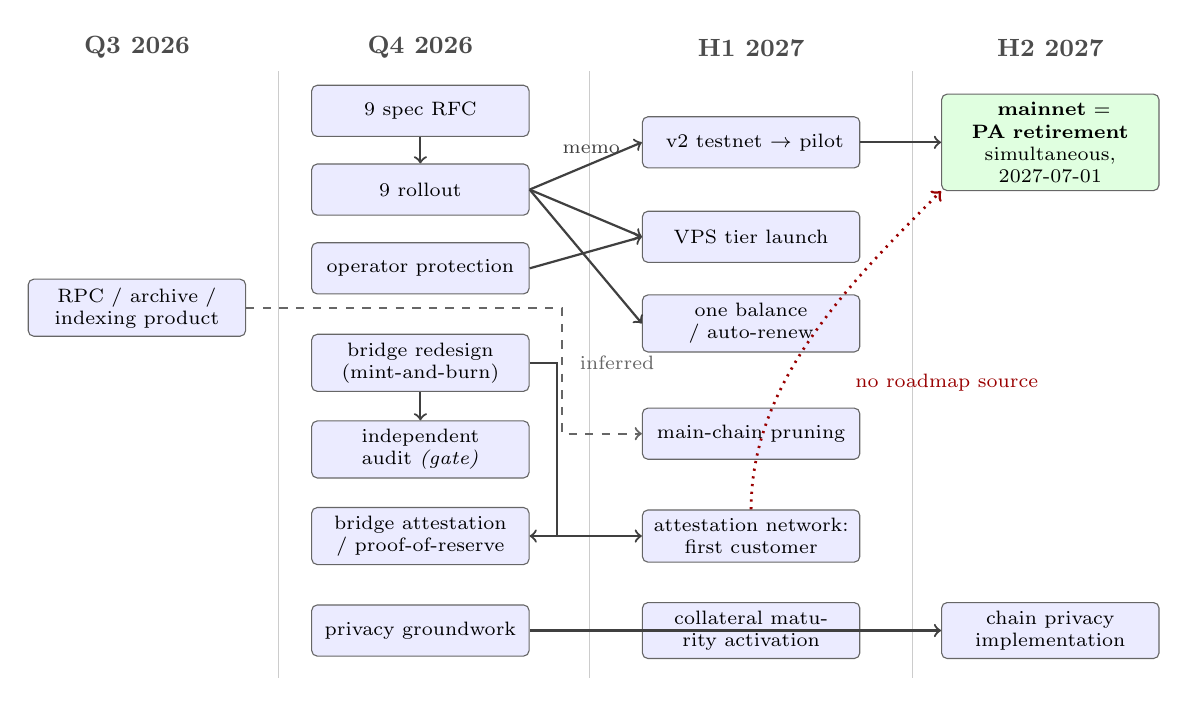
\begin{tikzpicture}[font=\scriptsize,
  n/.style={draw=black!60, rounded corners=2pt, fill=blue!8, align=center, inner sep=3pt,
            text width=2.55cm, minimum height=6.5mm},
  lane/.style={font=\small\bfseries, text=black!70},
  st/.style={->, thick, black!75},
  inf/.style={->, thick, black!60, dashed},
  unc/.style={->, thick, red!60!black, dotted, line width=1pt},
]
\node[lane] at (0,7.4)   {Q3 2026};
\node[lane] at (3.6,7.4) {Q4 2026};
\node[lane] at (7.8,7.4) {H1 2027};
\node[lane] at (11.6,7.4){H2 2027};
\draw[black!20] (1.8,-0.6) -- (1.8,7.1);
\draw[black!20] (5.75,-0.6) -- (5.75,7.1);
\draw[black!20] (9.85,-0.6) -- (9.85,7.1);

% Q3
\node[n] (rpc)  at (0,4.1) {RPC / archive / indexing product};
% Q4
\node[n] (rfc)  at (3.6,6.6) {\specv{9} spec RFC};
\node[n] (v9)   at (3.6,5.6) {\specv{9} rollout};
\node[n] (opro) at (3.6,4.6) {operator protection};
\node[n] (brd)  at (3.6,3.4) {bridge redesign (mint-and-burn)};
\node[n] (aud)  at (3.6,2.3) {independent audit \emph{(gate)}};
\node[n] (att4) at (3.6,1.2) {bridge attestation / proof-of-reserve};
\node[n] (priv) at (3.6,0.0) {privacy groundwork};
% H1
\node[n] (pnr)  at (7.8,6.2) {\PNR{} v2 testnet $\to$ pilot};
\node[n] (vps)  at (7.8,5.0) {VPS tier launch};
\node[n] (bal)  at (7.8,3.9) {one balance / auto-renew};
\node[n] (attn) at (7.8,1.2) {attestation network: first customer};
\node[n] (prun) at (7.8,2.5) {main-chain pruning};
\node[n] (coll) at (7.8,0.0) {collateral maturity activation};
% H2 / resolved
\node[n, fill=green!12] (act) at (11.6,6.2)
  {\textbf{\PNR{} mainnet $=$ PA retirement}\\{\scriptsize simultaneous, 2027-07-01}};
\node[n] (chpr) at (11.6,0.0) {chain privacy implementation};

\draw[st] (rfc) -- (v9);
\draw[st] (v9.east) -- node[above, pos=.55] {memo} (pnr.west);
\draw[st] (v9.east) -- (vps.west);
\draw[st] (v9.east) -- (bal.west);
\draw[st] (opro.east) -- (vps.west);
\draw[st] (brd) -- (aud);
\draw[st] (brd.east) -- ++(0.35,0) |- (att4.east);
\draw[st] (att4.east) -- (attn.west);
\draw[st] (priv.east) -- (chpr.west);
\draw[st] (pnr.east) -- (act.west);
%% The straight rpc->prun line crossed x=3.6 at y=3.36, i.e. through the middle of
%% `brd', and carried its label there. Routed instead along the clear corridor at
%% y=4.1 between `opro' (4.6) and `brd' (3.4), with the label on the vertical leg.
\draw[inf] (rpc.east) -- (5.4,4.1) -- (5.4,2.5) -- (prun.west);
\node[anchor=west, text=black!60] at (5.5,3.4) {inferred};
\draw[unc] (attn.north) .. controls +(0,1.6) and +(-1.2,-1.2) .. (act.south west);
\node[text=red!60!black, anchor=west] at (9.0,3.15) {no roadmap source};
\end{tikzpicture}
\caption{Roadmap dependency graph, oriented by quarter.}
\label{fig:dep-graph}
\end{figure}

\subsection{The edge that shapes the schedule: attestation alongside revenue}\label{sec:26-precondition}

\PNR pays all nodes from a shared fee pool through the \PoN rotation rather than paying the node
that hosts a given application (\planned; \srcintent{design intake}). A node's income is therefore
independent of \emph{which} applications it hosts. That is not free-riding, because an operator
cannot decline placement --- \FluxOS{}'s spawner selects at random from the network-wide list and no
opt-out exists (\shipped;
\srccode{flux/\allowbreak{}ZelBack/\allowbreak{}src/\allowbreak{}services/\allowbreak{}appLifecycle/\allowbreak{}appSpawner.js}{311}) ---
but it does mean \PNR supplies no gradient that rewards hosting well
(\planned; \srcintent{mechanism specification} \srcdoc{reconciliation record}). What compels a node to perform, in this design, is not \PNR — it is the eligibility gate
that lets a node participate in the \PoN rotation in the first place: benchmarking and attestation
(\S\ref{sec:consensus}, \S\ref{sec:attestation}). Those sections already establish that this gate is
weaker than it looks. The benchmark result \fluxd\ accepts is signed by network-wide shared keys
compiled into every copy of \fluxbench, not by a key bound to the operator who ran it (\shipped;
\srccode{fluxd/\allowbreak{}src/\allowbreak{}chainparams.cpp}{233--238}). The attestation key \fluxsas\ produces is derived
by HKDF from static salt and domain values compiled identically into every binary, with no input
that depends on a TPM, on Secure Boot state, or on any other per-machine value (\shipped;
\srcprivate{\SAS{} API server}). Neither signature is bound to the operator or the
machine that produced it.

These two findings compose badly, and the composition has to be sized before it can be turned into a
schedule. Because \PNR raises the value of holding an eligible, paying slot in the rotation, and
because passing the eligibility gate does not currently require possessing the hardware or operator
identity the gate is supposed to attest, \PNR raises the payoff to passing that gate without doing the
work, by exactly what it pays (\planned; \srcdoc{reconciliation record}).

\textbf{By how much is the question, and the answer bounds the conclusion.} At activation \PNR would
pay \num{286320}\flux\ per year. Operator issuance through the same gate at the same height is
\num{6386040}\flux\ per year (\S\ref{sec:pnr}). \PNR would raise the prize by \SI{4.5}{\percent}. An
earlier draft of this subsection concluded from the qualitative composition that hardening attestation
is a \emph{precondition} for \PNR mainnet activation; that conclusion does not survive the
arithmetic, and this paper withdraws it in favour of two statements that do.

\begin{enumerate}
  \item \textbf{Attestation hardening is the schedule's highest-priority security item on its own
  merits.} \SI{95.7}{\percent} of the income flowing through the unbound gate at activation is
  issuance that flows through it today. Treating the work as a \PNR dependency understates its
  urgency by more than an order of magnitude, and invites the reply --- correctly --- that a
  \SI{4.3}{\percent} supplement is not worth blocking a network upgrade for.
  \item \textbf{\PNR's ramp, not its activation, is what should track that work.} $\nodeshare$ rises
  from \num{0.20} to \num{0.50} over six reductions, and each step moves a larger share of operator
  income behind the gate. Coupling the ramp to attestation's completion prices the dependency where
  it actually grows, costs nothing at activation, and does not hand an opponent of \PNR a principled
  veto over it.
\end{enumerate}

What makes the coupling achievable rather than rhetorical is a finding recorded in
\S\ref{sec:attestation}: the image-bound TPM policy the hardening needs is \emph{already generated} on
every capable machine and simply has no consumer. The dependency is therefore not the roadmap's
opt-in bonded network with $k$-of-$n$ challengeable claims (\planned;
\srcroadmap{flux-roadmap-public.md:135-138}), which is a larger and later object, but the narrower
piece of work of binding the attestation key to that policy and serving a verifiable quote. Stated
that way the dependency and \PNR's own March-2027 activation height are compatible; stated as a
dependency on the bonded network, they are not, and the paper would be committing to two things that
conflict. The final row of Table~\ref{tab:dep-graph} is read accordingly.

\subsection{The second critical path: \specv{9}}\label{sec:26-v9}

FluxOS \specv{9} is the second critical path, and it is broader than \PNR alone. \PNR's fee-pool
memo depends directly on the v9 \texttt{paymentMemo} field (\planned; \srcroadmap{flux-roadmap-public.md:64,119}).
Deposited credits depend on the same substrate through the v9 \texttt{duration} field, and both
credits and the provisioning API's spending bounds depend further on a bounded-spending primitive
that \specv{9} does not by itself supply (\planned; \srcdoc{feasibility assessment, rows 1, 11, 14}). The
datacenter tier and the one-provider-runtime convergence depend on the v9 \texttt{machineType} flag
(\planned; \srcroadmap{flux-roadmap-public.md:64,125}; \srcdoc{feasibility assessment, row 21}).

Three of the fields this depends on have zero consumer code anywhere in \FluxOS today:
\texttt{paymentMemo}, \texttt{referralCode}, and \texttt{machineType} (\inprogress;
\srcdoc{reconciliation record}). The orchestration substrate of v9 is built and tested — 932 changed
files and a regression suite of 289 unit-test files running 7,763 test cases on every push
(\inprogress; \srcdoc{reconciliation record}) — but the economic fields the roadmap's own dependency
chain rests on are declared in the schema and unimplemented beneath it. The currently enforced
specification version remains \specv{8}, and 322 of 1{,}195 deployed applications (26.9\%) sit on
six versions older than that (\inprogress; \srcdoc{reconciliation record}; \srcmeasured{network census, \S5}{2026-09-03}).

The v9 enforcement height, settled at $\hstar = \num{3050000}$ (\S\ref{sec:appspec-v9}), is
therefore the most schedule-relevant date in this document (\srcdoc{feasibility assessment}). Meeting it
requires two things that do not exist yet: implemented consumers for the payment-memo, referral, and
machine-type fields, and \texttt{latest\allowbreak{}Supported\allowbreak{}Spec\allowbreak{}Version} raised in lockstep with a fleet-wide
version floor. The mastership/active-standby quorum plane, whose gating field
(\texttt{quorum\allowbreak{}Grant\allowbreak{}Activation\allowbreak{}Height}) is read by production code today but set only in test fixtures
(\inprogress; \srcdoc{reconciliation record}), is deliberately decoupled from $\hstar$ and activates
later, once \specv{9} is stable (\S\ref{sec:appspec-v9}). \settlednote{Partly. \specv{9} activation
and the migration of existing applications are both stated for \textbf{Q4~2026}
\srcintent{design intake}, the enforcement height is $\hstar = \num{3050000}$
\srcintent{design intake}, constrained to follow the economic-field implementation
(\Cref{rem:v9-timing}), and the migration policy is that all applications are migrated automatically
rather than by owner action \srcintent{design intake}. What remains open is the
mechanism by which the 322 applications on legacy versions are rewritten --- an automatic migration
still needs a specified transformation per source version, and none is stated in any artefact read
for this paper.}

\subsection{The privacy prerequisite}\label{sec:26-privacy}

Since height 835{,}554, \fluxd\ rejects any transaction that combines transparent inputs with a
shielded output or joinsplit, with the in-source comment stating the intent directly — the shielded
pool has accepted no new value in approximately 5.4 years (\shipped; \srccode{fluxd/\allowbreak{}src/\allowbreak{}main.cpp}{1398-1408}).
Value can leave the pool ($z \to t$) or move within it ($z \to z$), but it cannot enter.

\textbf{This prerequisite has been withdrawn, not scheduled.} An earlier round of the design intake
recorded that $t \to z$ would be reopened as part of a privacy update, and this paper carried it as a
scheduled dependency for wallet integration and for the payment path of
\S\ref{sec:private-payment}. That has been superseded: the team has decided to \textbf{retire both
shielded pools} rather than reopen either \srcintent{design intake} (\planned).
The reasoning and the schedule are in \S\ref{sec:shielded-retirement}; the consequence for this
section is that reopening leaves the migration path entirely.

Three items therefore leave the dependency graph rather than moving within it: the reopening
activation height, wallet integration for shielded sends in Zelcore and SSP, and the construction in
\S\ref{sec:private-payment} that would have consumed newly-entered value. One item is added: a
sunset height $\hshield = \num{3600000}$ after which shielded spends are invalid, together
with the outreach that must precede it (\S\ref{sec:shielded-retirement}). The roadmap's published direction --- ``we are bringing private
transactions back'' \srcroadmap{flux-roadmap-public.md:167}, and ``chain privacy implementation'' in
H2 2027 \srcroadmap{flux-roadmap-public.md:158} --- is superseded by this decision, and the paper
records the supersession rather than silently reinterpreting the roadmap. What the roadmap says about
not pinning a date on a cryptographic change before its audit is scoped
\srcroadmap{flux-roadmap-public.md:177} still applies, and now applies to a possible \emph{future}
shielded construction (\S\ref{sec:orchard-migration}) rather than to a reopening.

\subsection{The activation schedule}\label{sec:26-schedule}

Table~\ref{tab:activation-schedule} reproduces the design intake's activation schedule: block
height, calendar date, \PoN subsidy $\subsidypon$, and node share $\nodeshare$ through the ramp
toward the cap $\nodesharecap = 50\%$ (\planned; \srcintent{design intake}).

\begin{table}[H]
\centering
\small
\begin{tabular}{@{}lrlrl@{}}
\toprule
Event & Height & Date & Subsidy ($\subsidypon$, \flux) & Node share ($\nodeshare$) \\
\midrule
Current & $\sim$2{,}912{,}015 & 2026-09-03 & 14.0 & --- \\
Reduction 1 ($-10\%$) & 3{,}071{,}200 & 2026-10-25 & 12.6 & --- \\
PA Depletion ($-50\%$), $\hpa$ & \textbf{3{,}787{,}502} & \textbf{2027-07-01} & \textbf{6.3} & \textbf{20\% --- \PNR begins} \\
Reduction 2 ($-10\%$) & 4{,}122{,}400 & 2027-10-25 & 5.67 & 25\% \\
Reduction 3 ($-10\%$) & 5{,}173{,}600 & 2028-10-24 & 5.103 & 30\% \\
annually thereafter & $+1{,}051{,}200$ & --- & $\times 0.9$ & $+5$pp \\
\bottomrule
\end{tabular}
\caption{\PNR activation schedule from the design intake. PA Depletion ($\hpa$) is simultaneous with
the parallel-asset mining-reward cut and the swap contract taking effect
(\S\ref{sec:26-schedule}; \srcintent{design intake}), not a half-year ahead of it as
the public roadmap's superseded sequencing would have had it. Node share $\nodeshare$ ramps to a
declared cap $\nodesharecap = 50\%$, reached around 2033 on the stated annual step
(\srcintent{design intake}).}
\label{tab:activation-schedule}
\end{table}

\PNR activation and the parallel-asset emission cut occur at the \emph{same} event: height
$\hpa = 3{,}787{,}502$, 2027-07-01, is when the node share $\nodeshare$ first becomes nonzero and when
parallel-asset mining-reward emission is cut (\planned; \srcintent{design intake}). This resolves what
earlier drafts of this paper carried as an open sequencing conflict (C1a). The public roadmap had
stated a different, sequential plan — ``retirement of any parallel asset's mining rewards comes only
after PNR v2 is demonstrably paying operators'' and, more specifically, ``parallel-asset mining
retirement — only after PNR v2 is paying operators on mainnet, announced at least 90 days ahead'' — a
step the roadmap placed in H2 2027, one half-year after PNR v2's own H1 2027 slot
(\srcroadmap{flux-roadmap-public.md:133,159}). That sequencing is \textbf{superseded} by the team's
direct answer to this paper: activation is simultaneous, at $\hpa$ (\planned;
\srcintent{design intake}). This section and \S\ref{sec:parallel-assets} both now
describe one coordinated transition rather than two phases separated by an interval.

The consequence is not merely notational. The roadmap's sequential design existed to create a
checkpoint: a proving period, of up to a stated half-year with 90 days' advance notice, in which
\PNR could be observed actually paying operators before the parallel assets whose retirement it was
meant to justify were cut. With simultaneous activation, that checkpoint does not exist —
deliberately, by the team's own later decision, not by oversight. \S\ref{sec:26-risk} carries this as
a named risk rather than treating the superseded roadmap language as still in force.

\subsection{An empirical base rate for consensus change}\label{sec:26-basrate}

The transition this paper's thesis rests on was not clean, and the fact belongs in a risk analysis
rather than a footnote. \fluxd's normal reorg-depth limit, \texttt{MAX\_REORG\_LENGTH}, is 40
blocks, but it was overridden to 5{,}000 for the height range $[2{,}020{,}000,\ 2{,}025{,}000]$, an
override the source comments describe as a ``[t]emporary deep reorg limit during PON stabilization
period'' (\shipped; \srccode{fluxd/\allowbreak{}src/\allowbreak{}main.cpp}{8983-8988}). Alongside it sits a checkpoint cluster
at heights 2{,}020{,}500 / 2{,}021{,}000 / 2{,}021{,}500 / 2{,}022{,}000 / 2{,}029{,}000, labelled in
the source ``PON activation and stabilization checkpoints -- EMERGENCY FORK RECOVERY'' (\shipped;
\srccode{fluxd/\allowbreak{}src/\allowbreak{}chainparams.cpp}{277-283}). The \PoW$\to$\PoN transition, in other words, required
active emergency intervention after activation despite having been planned.

The roadmap itself draws two lessons from this kind of history, applied prospectively to the next
consensus change it proposes (collateral maturity): first, that a proposal should ride an
already-planned network upgrade rather than force its own — ``it would ride an already-planned
network upgrade rather than forcing its own'' (\planned; \srcroadmap{flux-roadmap-public.md:146});
second, that proposals go to operators for discussion before any activation is scheduled, not after
— stated for collateral maturity (\srcroadmap{flux-roadmap-public.md:146}) and echoed in \PNR's own
staged sequence, which ends with ``per-tier before-and-after examples published to operators before
activation'' (\planned; \srcroadmap{flux-roadmap-public.md:119}). Three further consensus-adjacent
changes are queued behind \PoN and sit in \S\ref{sec:chain-ops}: main-chain pruning (\planned;
\srcroadmap{flux-roadmap-public.md:121-122}), collateral maturity (\planned;
\srcroadmap{flux-roadmap-public.md:143-146}), and the post-quantum migration roadmap (\planned;
\srcroadmap{flux-roadmap-public.md:148-149}) — the last of which the roadmap is explicit is a
multi-year effort beyond publishing a path. Against the C16 base rate, this is why sequencing them
into as few network upgrades as possible matters: each additional independently-forced consensus
change is, by the network's own recent history, an occasion on which stabilization measures of the
kind seen at \PoN activation may again be needed.

\subsection{Risk register}\label{sec:26-risk}

Table~\ref{tab:risk-register} lists the risks this section's dependency analysis surfaces, the
mechanism each threatens, the evidence behind its likelihood, and the mitigation that exists or does
not.

%% longtable rather than table[H]: the [H] tabular ran 272pt past the text block (log: overfull
%% vbox), so its last row was cut and its caption never rendered. Same header pattern as Appendix B.
\begingroup
\footnotesize
\begin{longtable}{@{}p{2.9cm}p{2.1cm}p{4.3cm}p{3.6cm}@{}}
\caption{Risk register for the sequencing and dependencies described in this section.}
\label{tab:risk-register}\\
\toprule
Risk & Threatens & Likelihood basis (evidence) & Mitigation \\
\midrule
\endfirsthead
\multicolumn{4}{l}{\small\itshape (Table~\ref{tab:risk-register} continued)}\\
\toprule
Risk & Threatens & Likelihood basis (evidence) & Mitigation \\
\midrule
\endhead
\bottomrule
\endfoot
Demand growth undershoots; \PNR stays a supplement & \PNR (\S\ref{sec:pnr}) &
At $\hpa$, parity needs $\sim$31.9M\flux/yr (\S\ref{sec:eval-pnr-crossover}) against assumed demand
of $\sim$1.43M\flux/yr (the team's assumption of 1{,}193 applications at 100\flux/month; the census
counts 1{,}195 applications and 7{,}486 instances, \S\ref{sec:eval-apps}); \PNR is $\sim$4.3\% of
operator income at activation; under flat demand there is no crossover, ever (\srcintent{design intake};
\srcdoc{reconciliation record}) &
Ramp lowers the parity threshold to $\sim$6.8M\flux/yr by 2032-10, $\sim$5.6 years post-$\hpa$
(\S\ref{sec:eval-pnr-crossover}); no stated policy if demand still undershoots (O13, open) \\
\addlinespace
Simultaneous activation removes the roadmap's proving-period checkpoint & \PNR credibility;
parallel-asset retirement (\S\ref{sec:pa-sequencing}, \S\ref{sec:26-schedule}) &
\PNR activation and the parallel-asset emission cut are simultaneous at $\hpa = 3{,}787{,}502$
(\srcintent{design intake}), superseding the roadmap's plan to retire parallel
assets only after \PNR is ``demonstrably paying operators,'' announced 90 days ahead
(\srcroadmap{flux-roadmap-public.md:133,159}) &
None stated; a deliberate simplification by the team, not an oversight, but it means no external
observer can verify \PNR is paying operators before the parallel assets it justifies retiring are cut \\
\addlinespace
Eligibility-gate exploitation once \PNR pays & \PNR's only hosting compulsion (\S\ref{sec:consensus},
\S\ref{sec:attestation}) &
Benchmark keys are shared constants, not per-operator (\srccode{fluxd/\allowbreak{}src/\allowbreak{}chainparams.cpp}{233--238});
attestation key derivation has no machine-bound input (\srcprivate{\SAS{} API server});
\PNR{} adds no gradient rewarding good hosting (\srcdoc{reconciliation record}), though it adds only
\SI{4.5}{\percent} to a payoff the same gate already carries &
Machine-binding the attestation key to the PCR 4/7/11 policy \ArcaneOS{} already generates
(\S\ref{sec:attestation}) --- narrower and nearer than the roadmap's opt-in bonded network, k-of-n,
planned H1 2027 (\srcroadmap{flux-roadmap-public.md:135-138}); \S\ref{sec:26-precondition} couples it
to \PNR's ramp rather than blocking activation on it \\
\addlinespace
A bridge audit finding delays consolidation & Bridge redesign, chain consolidation (\S\ref{sec:bridge}) &
Audit is an explicit hard gate before deploy (\srcroadmap{flux-roadmap-public.md:97}); the network's
only prior consensus-adjacent transition needed emergency intervention despite planning
(\S\ref{sec:26-basrate}) &
Audit-before-deploy is itself the stated mitigation; no contingency schedule exists for a finding
that requires rework (open) \\
\addlinespace
\specv{9} migration strands legacy applications & \PNR, credits, provisioning API, datacenter tier
(\S\ref{sec:26-v9}) &
322 of 1{,}195 deployed applications (26.9\%) sit on six versions older than \specv{8}
(\srcdoc{reconciliation record}; \srcmeasured{network census, \S5}{2026-09-03}); the enforcement
height is settled at $\hstar = \num{3050000}$ but no per-version transformation or eviction
policy exists &
Forced automatic migration at $\hstar$ \srcintent{design intake}; the
transformation per source version is unspecified (\S\ref{sec:26-v9}) \\
\addlinespace
Moderation-quorum capture event & Content-reporting quorum (\S\ref{sec:governance}) &
4 owner identities (\texttt{payment\_address}) reach the 25\% eviction threshold, falling to 3 once addresses linked by a shared node key or collateral funding transaction are merged; the largest holds 10.71\% of collateral-weighted
voting power; Gini 0.8375 (\srcmeasured{network census, \S2}{2026-09-03}; \srcdoc{reconciliation record}) &
Two-chamber rule (weight threshold plus distinct-identity count with tenure) raises the cost of a
surprise capture but does not lower $\kappa$; does not reach censorship resistance (\srcdoc{reconciliation record}) \\
\addlinespace
Shielded-pool sunset destroys notes not swept in time & Holders of the 96{,}479.94\flux{} still in
the pools (\S\ref{sec:privacy}, \S\ref{sec:shielded-retirement}) &
$t \to z$ closed since height 835{,}554, approximately 5.4 years (\srccode{fluxd/\allowbreak{}src/\allowbreak{}main.cpp}{1398-1408});
reopening is cancelled and both pools are to be retired
(\srcintent{design intake}); roadmap will not pin a date on a cryptographic
change before its audit is scoped (\srcroadmap{flux-roadmap-public.md:177}) &
Sunset settled at $\hshield = \num{3600000}$ (2027-04-27), announced at publication and \num{187502} blocks before $\hpa$
(\srcintent{design intake}); ZIP-209 turnstile enforcement active for the window
and direct holder outreach are this paper's recommendations, not confirmed decisions
(\S\ref{sec:shielded-retirement}) \\
\addlinespace
Archival capacity becomes demand-dependent once history is a paid product & Pruning, archive/RPC/indexing
(\S\ref{sec:chain-ops}, \S\ref{sec:managed-services}) &
Roadmap pairs the Q3 2026 archive product directly with H1 2027 pruning, but states the direction
loosely and marks it \srcinferred\ in its own dependency list rather than as a strict gate
(\srcroadmap{flux-roadmap-public.md:34,121-122}) &
None stated; if the archive product does not attract paying demand, the operator incentive to run
archive nodes once pruning removes the default full-history requirement is untested \\
\end{longtable}
\endgroup

\subsection{What would have to be true}\label{sec:26-conditions}

This is not a schedule with a confidence interval attached; it is a set of conditions, stated
explicitly, under which the sequencing above resolves into a working rollout rather than a stalled
or exploited one.

\begin{itemize}
\item \textbf{Demand, not price, must grow.} The number of deployed applications, instances, and
resources sold must grow roughly in line with the compounding schedule in
Table~\ref{tab:activation-schedule} for \PNR to become more than a $\sim$4\% supplement to operator
income; this is a claim about deployment counts and resources sold, never about price
(\srcintent{design intake}; \srcdoc{reconciliation record}).
\item \textbf{Attestation hardening must precede or coincide with \PNR mainnet activation, not
follow it.} If the bonded attestation network is not operational by the time \PNR begins paying
operators, the eligibility gate — already shown not to be operator- or machine-bound
(\S\ref{sec:26-precondition}) — becomes a directly monetized target rather than a weak but
unexploited assumption.
\item \textbf{\specv{9}'s three economic fields need implemented consumers before any of their
dependents activate.} \texttt{paymentMemo}, \texttt{referralCode}, and \texttt{machineType} must
each acquire consumer code, and \texttt{latest\allowbreak{}Supported\allowbreak{}Spec\allowbreak{}Version} must rise in lockstep with a
fleet-wide version floor, before \PNR,
credits, the provisioning API's bounds, or the datacenter tier can activate on the schedule the
roadmap implies (\srcdoc{reconciliation record}).
\item \textbf{The shielded-pool sunset must be executed as settled.} Reopening $t \to z$ is cancelled and
both pools are to be retired \srcintent{design intake}; what replaces the old open
question is a sunset height $\hshield = \num{3600000}$, confirmed
\srcintent{design intake}, together with ZIP-209 turnstile enforcement for the
drain-only window and the direct outreach preceding it, both this paper's recommendations
(\S\ref{sec:shielded-retirement}, \S\ref{sec:26-privacy}).
\item \textbf{The removed proving period is an accepted risk, not an oversight, and should stay
visible.} Simultaneous activation (\S\ref{sec:26-schedule}) means no external observer can confirm
\PNR pays operators before parallel-asset mining rewards are retired; any activation announcement
should say so rather than let a reader assume the roadmap's original 90-day-notice checkpoint still
applies.
\item \textbf{Consensus changes need to be batched into as few network upgrades as possible},
following the roadmap's own stated preference to ride an already-planned upgrade rather than force a
new one; every additional independently-forced consensus change is, by the measured base rate of the
\PoW$\to$\PoN transition, an occasion on which unplanned stabilization measures may again be needed
(\S\ref{sec:26-basrate}).
\item \textbf{The bridge audit and the moderation quorum's residual capture risk need to be treated
as live constraints, not formalities}, since neither has a stated contingency for an adverse finding
or a captured vote (Table~\ref{tab:risk-register}).
\end{itemize}

%% Drain this section's float queue before the next begins.
\FloatBarrier
